
\section{Comparison with simplices}

In \cite[p. 442]{Serre1951homologie}, Serre described a quasi-isomorphism for any space between its simplicial and cubical singular chains. A chain map also considered in \cite[p.199]{Eilenberg1953acyclic} where it is attributed to Cartan.
To describe it let us consider the topological simplex
\begin{equation*}
\gsimplex^n = \{(y_0, \dots, y_n) \mid y_i \in [0,1], \ \textstyle{\sum} \, y_i = 1\}
\end{equation*}
and the topological cube
\begin{equation*}
\gcube^{n} = \{(x_1, \dots, x_n) \mid x_i \in [0,1]\}
\end{equation*}
with their usual CW structures.
The \textit{Cartan-Serre} \textit{map} $\gcube^n \to \gsimplex^n$ is defined by
\begin{equation} \label{e:cartan-serre CW map}
\begin{split}
&y_0 = 1 - x_1, \\
&y_1 = x_1(1 - x_2), \\
&\ \vdots \\
&y_{n-1} = x_1 x_2 \cdots x_{n-1}(1-x_n), \\
&y_{n} = x_1 x_2 \cdots x_n,
\end{split}
\end{equation}
and is such that, for any topological space $Z$, the induced chain map $\chains(\Sing^{\simplex} Z) \to \chains(\Sing^{\cube} Z)$ on singular chain complexes is a quasi-isomorphism.
Furthermore, Serre states that this chain map is ``comultiplicative", i.e., that it commutes with the Alexander-Whitney and Serre diagonals.
The goal of this section is to prove a generalization of this statement, showing that this map is a morphism of $E_\infty$ coalgebras.
We will deduce this result from a more general categorical statement.

The \textit{simplex category} $\simplex$ is the full subcategory of $\Cat$ with objects
\begin{equation*}
[n] = 0 \to 1 \to \cdots \to n.
\end{equation*}
Its morphisms are generated by the \textit{coface} and \textit{codegeneracy functors} defined by
\begin{align*}
...
\end{align*}

We denote by $\simplex_{\deg}$ the subcategory with the same objects as $\simplex$ and morphisms of the form $\sigma_i \circ \tau$ for some morphisms $\tau$ of $\simplex$.

The category of \textit{simplicial sets} is the functor category $\sSet = \Fun(\simplex^\op, \Set)$.
An important example is the singular complex $\Sing Z$ of a topological space.

The \textit{product} of simplicial sets is defined by
\begin{equation*}
(X \times Y)[n] = X[n] \times Y[n], \qquad
(X \times Y)(\tau) = X(\tau) \times Y(\tau).
\end{equation*}
For elements in $X \times Y$ we follow the convention of writing $x \times y$ instead of $(x, y)$.

The \textit{standard $n$-simplex} is the cubical set $\simplex^n = \simplex(-, [n])$.
The \textit{Yoneda embedding} $\simplex \to \sSet$ is the functor induced by $[n] \mapsto \simplex^n$, and for any simplicial set $X$ we have
\begin{equation*}
X[n] \cong \colim_{\simplex^n \to X} \simplex^n.
\end{equation*}

The functor of \textit{chains} $\cchains \colon \sSet \to \Ch$ is the Kan extension along the Yoneda embedding of the functor $\simplex \to \Ch$ assigning to $[n]$ the chain complex whose degree $m$ part is the $R$-module
\begin{equation*}
\frac{R\{\simplex([m], [n])\}}{R\{\simplex_{\deg}([m], [n])\}}
\end{equation*}
and whose boundary is defined by
\begin{equation*}
\partial (\id_{[n]}) = \sum_{i=0}^{n} (-1)^i \ \id_{[n]} \circ \delta_i.
\end{equation*}
We remark that $\chains(\simplex^n)$ is isomorphic to the cellular chains on $\gsimplex^n$.


In \cite{Medina20prop1}, a similar construction to the one introduced in Section~\ref{s:coaction} provides the chains of simplicial sets with a natural $U(\M)$-coalgebra structure.
It is also induced from a natural $\M$-bialgebra structure on the chains of standard simplices.
This $\M$-bialgebra structure on $\chains(\simplex^n)$ is defined by the assignment
\begin{equation*}
\counit \mapsto \epsilon, \quad \coproduct \mapsto \Delta, \quad \product \mapsto \ast,
\end{equation*}
where
\begin{equation*}
\varepsilon \big( [v_0, \dots, v_q] \big) = \begin{cases} 1 & \text{ if } q = 0, \\ 0 & \text{ if } q > 0, \end{cases}
\end{equation*}
is the \textit{augmentation map},
\begin{equation*}
\Delta \big( [v_0, \dots, v_q] \big) = \sum_{i=0}^q [v_0, \dots, v_i] \otimes [v_i, \dots, v_q],
\end{equation*}
is the \textit{Alexander-Whitney diagonal}, and the following is an algebraic version of the \textit{join}:
\begin{equation*}
\left[v_0, \dots, v_p \right] \ast \left[v_{p+1}, \dots, v_q\right] = \begin{cases} (-1)^{p+|\pi|} \left[v_{\pi(0)}, \dots, v_{\pi(q)}\right] & \text{ if } v_i \neq v_j \text{ for } i \neq j, \\
0 & \text{ if not}, \end{cases}
\end{equation*}
where $\pi$ is the permutation that orders the totally ordered set of vertices and $(-1)^{|\pi|}$ is its sign.

We will make $S$ into an $E_\infty$ bialgebra map by restricting the $\M$-bialgebra structures on $\cchains(\cube^n)$ and $\chains(\simplex^n)$ to an $E_\infty$ sub-prop of $\M$ which we now describe.

We will utilize the following diagrammatic simplification
\begin{center}
	\boxed{\begin{tikzpicture}[scale=.4]
		\draw (6,2)--(7,1)--(7,0);
		\draw (8,2)--(7,1);
		\node at (6,2.5){$\scriptstyle 1$};
		\node at (7,2.5){$\scriptstyle \dots$};
		\node at (8,2.5){$\scriptstyle n$};
		
		\draw (11,.5)--(12,1.5)--(12,2.5);
		\draw (13,.5)--(12,1.5);
		\node at (11,0){$\scriptstyle 1$};
		\node at (12,0){$\scriptstyle \dots$};
		\node at (13,0){$\scriptstyle n$};
		\end{tikzpicture}}
\end{center}
to represent labeled directed graphs resulting from iterated grafting of \product and \coproduct \ in the left comb order
\begin{center}
	\boxed{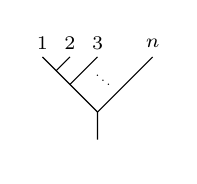
\begin{tikzpicture}[scale=.35]		
		\node at (-2.15,-.25){};
		\node at (-2.15,3.25){};
		
		\node at (-2,3.5){$\scriptstyle 1$};
		\node at (-1,3.5){$\scriptstyle 2$};
		\node at (0,3.5){$\scriptstyle 3$};
		\node at (2,3.5){$\scriptstyle n$};
		
		\draw (-2,3)--(0,1);
		\draw (2,3)--(0,1)--(0,0);
		\draw (0,3)--(-1,2);
		\draw (-1,3)--(-1.5,2.5);
		\draw (.2,2.3) node[scale= 0.5] {$\ddots$};
		\end{tikzpicture}
		\qquad 
		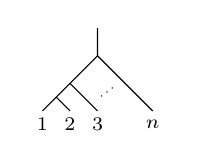
\begin{tikzpicture}[scale=.35]	
		
		\node at (-2,-3.5){$\scriptstyle 1$};
		\node at (-1,-3.5){$\scriptstyle 2$};
		\node at (0,-3.5){$\scriptstyle 3$};
		\node at (2,-3.5){$\scriptstyle n$};
		
		\draw (-2,-3)--(0,-1);
		\draw (2,-3)--(0,-1)--(0,0);
		\draw (0,-3)--(-1,-2);
		\draw (-1,-3)--(-1.5,-2.5);
		\draw (.2,-2.3) node[scale= 0.5, rotate = 75] {$\ddots$};
		\end{tikzpicture}}
\end{center}

A \textit{surjection-like graph} is either the $(1,0)$-graph \counit\ or for $n > 1$ a $(1, n)$-graph of the form 
\begin{center}
\boxed{\begin{tikzpicture}[scale=.4]
	\node at (5,8){$\scriptstyle 1$};
	\draw (3,5.5)--(5,6.5)--(5,7.5);
	\draw (7,5.5)--(5,6.5);
	\node at (3,5){$\scriptstyle 1$};
	\node at (5,5){\,$\scriptstyle \dots$};
	\node at (7,5){$\scriptstyle r+d$};
	
	\node at (5,4){$\vdots$};
	
	\node at (3,-.5){$\scriptstyle 1$};
	\draw (2,2)--(3,1)--(3,0);
	\draw (4,2)--(3,1);
	\node at (2,2.5){$\scriptstyle 1$};
	\node at (3,2.5){$\scriptstyle \dots$};
	\node at (4,2.5){$\scriptstyle k_1$};
	
	\node at (5,1){\ $\cdots$};
	
	\node at (7,-.5){$\scriptstyle r$};
	\draw (6,2)--(7,1)--(7,0);
	\draw (8,2)--(7,1);
	\node at (6,2.5){$\scriptstyle 1$};
	\node at (7,2.5){$\scriptstyle \dots$};
	\node at (8,2.5){$\scriptstyle k_r$};
	\end{tikzpicture}}
\end{center}
containing no internal vertices and such that for each $i = 1, \dots, r$ the induced map 
\begin{equation*}
\{1, \dots, k_i\} \to \{1, \dots, r+d\}
\end{equation*}
is order preserving.

\begin{definition}
	The prop $\MS$ is the sub-prop of $\M$ generated by elements represented by surjection-like graphs.
\end{definition}

The same proof used in \cite[Theorem 3.3.]{Medina20prop1} shows $\MS$ is an $E_\infty$ prop.
The associated operad $U(\MS)$ was used in \cite[Theorem A.11.]{Medina20prop1} to compare the action of the surjection operad of McClure-Smith \cite{mcclure2003multivariable} and Berger-Fresse \cite{berger2004combinatorial} on simplicial sets and that of $U(\M)$.

By restricting their respective $\M$-bialgebra structures to $\MS$-bialgebra structure we have that both $\chains \cube^n$ and $\chains \simplex^n$ are $\MS$-bialgebras.
This restriction is important for comparing these structures as we describe next.

\subsection{Comparison}

%The Cartan-Serre chain map $S$ is not in general a morphism of $\M$-bialgebras, for example, notice that $S([0] \otimes [0,1]) = 0$, but $([1] \otimes [1]) \ast ([0] \otimes [0,1]) = -([0,1] \otimes [0,1])$ which is mapped to $-[0,1,2]$ by $S$.

For non-negative integers $n$ and $m$, we identify the set $\simplex^n_m$ with that of non-decreasing sequences $[v_0, \dots, v_m]$ with each $v_i \in \{0, \dots, n\}$.
For $\simplex^1_m = \simplex([m], [1])$ we reduce notation writing
\begin{equation*}
\langle k \rangle = [\, \overbrace{0,\dots,0}^{m+1-k}, \overbrace{1,\dots,1}^{k}\,]
\end{equation*}
for $k \in \{0, \dots, m+1\}$

%\begin{equation*}
%\big\{ \langle k \rangle = [\, \overbrace{0,\dots,0}^{m+1-k}, \overbrace{1,\dots,1}^{k}\,] \mid k \in \{0, \dots, m+1\} \big\}
%\end{equation*}
%with degeneracy and face maps given by repeating and removing entries respectively.
%It can be given a total order lexicographically, making the assignment $k \mapsto \angles{k}$ into an order-preserving map.

Let us now consider the product $\scube{n}$ with
\begin{equation*}
\scube{n}_m = \big\{ \angles{k_1} \times \cdots \times \angles{k_n} \mid \angles{k_i} \in \simplex^1_m \big\}.
\end{equation*}
For $n \in \{0,1\}$, the simplicial sets $\simplex^n$ and $\scube{n}$ are isomorphic.
For $n > 1$ we consider the inclusion of simplicial sets
\begin{equation*}
\begin{tikzcd}[row sep=-3pt, column sep=small,
/tikz/column 1/.append style={anchor=base east},
/tikz/column 2/.append style={anchor=base west}]
\simplex^n \arrow[r, "\iota"] & \scube{n} \\
{[0, \dots, n]} \arrow[r, mapsto] & \angles{n} \times \cdots \times \angles{1},
\end{tikzcd}
\end{equation*}
and the projection of simplicial sets $s \colon \scube{n} \to \iota(\simplex^n)$ defined by
\begin{equation*}
[ \varepsilon_0^1, \dots, \varepsilon_m^1] \times \cdots \times [ \varepsilon_0^n, \dots, \varepsilon_m^n] \mapsto [ \eta_0^1, \dots, \eta_m^1] \times \cdots \times [ \eta_0^n, \dots, \eta_m^n]
\end{equation*}
with $\eta_i^k = \varepsilon_i^1 \cdots \varepsilon_i^k$, or, recursively, by
\begin{equation*}
s\big(\angles{k_1} \times \cdots \times \angles{k_n}\big) =
\begin{cases}
\angles{k_1} \times s\big(\angles{k_2} \times \cdots \times \angles{k_n}\big) & k_1 \geq k_2, \\
\angles{k_1} \times s\big(\angles{k_1} \times \cdots \times \angles{k_n}\big) & k_1 < k_2.
\end{cases}
\end{equation*} 
The inclusion $\iota$ is a section of $s$, i.e., it satisfies $s \circ \iota = \id_{\simplex^n}$.

The assignment $2^n \mapsto \scube{n}$ defines a functor $\cube \to \sSet$ with $\delta_i^\varepsilon$ inserting $[\varepsilon, \dots, \varepsilon]$ in the $i\th$ position, and $\sigma_i$ removing the $i\th$ factor.
The left Kan extension of this functor $\T \colon \cSet \to \sSet$, referred to as \textit{triangulation}, admits a right adjoint $\U \colon \sSet \to \cSet$ defined by
\begin{equation*}
(\U X)(2^m) = \sSet \big( \scube{n}, \, X \big).
\end{equation*}
Although we do not use this fact, we mention that $\T$ and $\U$ define a Quillen equivalence when simplicial and cubical sets are considered as model categories in the usual way \cite[8.4.30]{cisinski2006presheaves}.

For any simplicial set $Y$ the map $s \colon \scube{n} \to \simplex^n$ induces a map
\begin{equation*}
\begin{tikzcd}[column sep = small, row sep=tiny]
\sSet(\simplex^n, Y) \arrow[r] &
\sSet(\T \cube^n, Y) \\
\big( \simplex^n \stackrel{g}{\to} Y \big) \arrow[r, maps to] &
\big(\scube{n} \stackrel{s}{\to} \simplex^n \stackrel{g}{\to} Y \big),
\end{tikzcd}
\end{equation*}
for every $n \geq 0$, which, composing with the adjunction isomorphism, gives a map
\begin{equation*}
\begin{tikzcd}[column sep = small, row sep=tiny]
\sSet(\simplex^n, Y) \arrow[r] &
\cSet(\cube^n,\, \U Y) \\
\big( \simplex^n \stackrel{g}{\to} Y \big) \arrow[r, maps to] &
\Big(\cube^n \stackrel{\T}{\to} \big(\scube{n} \stackrel{g \circ s\,}{\, \longrightarrow\, } Y \big)\Big).
\end{tikzcd}
\end{equation*}
These define a map of graded sets inducing a chain map $S \colon \chains(Y) \to \chains(\U Y)$, which is a quasi-isomorphism by an acyclic carrier argument.
This chain map is a morphisms of $E_\infty$ coalgebras.

\begin{theorem} \label{t:comparison}
	For any simplicial set $Y$ the chain map $S \colon \chains(Y) \to \chains(\U Y)$ is a morphisms of $U(\MS)$-coalgebras.
\end{theorem}

This follows from the next result.
Its proof occupies Section~\ref{s:proof2}.

\begin{lemma}
	The composition
	\begin{equation*}
	\begin{tikzcd}[column sep=normal]
	\chains \cube^n \arrow[r, "\chains \T"] &[-3pt] \chains \big( \scube{n} \big) \arrow[r, "\chains s"] &[-3pt] \chains \simplex^n
	\end{tikzcd}
	\end{equation*}
	is a morphism of $\MS$-bialgebras.
\end{lemma}

Using the identification of $\chains \cube^n$ and $\chains \simplex^n$ with the cellular chains of $\gcube^n$ and $\gsimplex^n$ respectively, one can verify that the chain map induced by the Cartan-Serre map $\gcube^n \to \gsimplex^n$ is equal to the above composition and we have the following consequence.

\begin{corollary}
	For any topological space, the quasi-isomorphism induced by the Serre-Cartan map from its singular simplicial chains to its singular cubical chains is a morphisms of $E_\infty$-coalgebras.
\end{corollary}